\documentclass[11pt,a4paper]{article}

% ============================================================
% Guía de usuario LaTeX
% AppImage Launcher Creator
% TECPROG WORLD E.I.R.L.
% ============================================================

\usepackage[utf8]{inputenc}
\usepackage[T1]{fontenc}
\usepackage[spanish]{babel}
\usepackage{geometry}
\usepackage{xcolor}
\usepackage{hyperref}
\usepackage{graphicx}
\usepackage{float}
\usepackage{longtable}
\usepackage{array}
\usepackage{booktabs}
\usepackage{fancyhdr}
\usepackage{titlesec}
\usepackage{listings}
\usepackage{enumitem}

\geometry{
    left=2.2cm,
    right=2.2cm,
    top=2.4cm,
    bottom=2.4cm
}

\definecolor{tecgreen}{HTML}{7FB239}
\definecolor{tecdark}{HTML}{111827}
\definecolor{tecgray}{HTML}{374151}
\definecolor{codebg}{HTML}{F3F4F6}
\definecolor{codeborder}{HTML}{CBD5E1}

\hypersetup{
    colorlinks=true,
    linkcolor=tecgreen,
    urlcolor=tecgreen,
    citecolor=tecgreen,
    pdftitle={Guía de usuario de AppImage Launcher Creator},
    pdfauthor={TECPROG WORLD E.I.R.L.}
}

\setlength{\headheight}{14pt}
\pagestyle{fancy}
\fancyhf{}
\lhead{\textbf{TECPROG WORLD E.I.R.L.}}
\rhead{\textbf{AppImage Launcher Creator}}
\cfoot{\thepage}

\titleformat{\section}
{\Large\bfseries\color{tecdark}}
{\thesection}{0.6em}{}

\titleformat{\subsection}
{\large\bfseries\color{tecgray}}
{\thesubsection}{0.6em}{}

\titleformat{\subsubsection}
{\normalsize\bfseries\color{tecgray}}
{\thesubsubsection}{0.6em}{}

\lstset{
    literate=
    {á}{{\'a}}1 {é}{{\'e}}1 {í}{{\'i}}1 {ó}{{\'o}}1 {ú}{{\'u}}1
    {Á}{{\'A}}1 {É}{{\'E}}1 {Í}{{\'I}}1 {Ó}{{\'O}}1 {Ú}{{\'U}}1
    {ñ}{{\~n}}1 {Ñ}{{\~N}}1
    {ü}{{\"u}}1 {Ü}{{\"U}}1
    {¿}{{?`}}1 {¡}{{!`}}1
}

\lstdefinestyle{bashstyle}{
    backgroundcolor=\color{codebg},
    basicstyle=\ttfamily\small,
    breaklines=true,
    frame=single,
    rulecolor=\color{codeborder},
    columns=fullflexible,
    keepspaces=true,
    showstringspaces=false,
    tabsize=4,
    language=bash
}

\lstdefinestyle{textstyle}{
    backgroundcolor=\color{codebg},
    basicstyle=\ttfamily\small,
    breaklines=true,
    frame=single,
    rulecolor=\color{codeborder},
    columns=fullflexible,
    keepspaces=true,
    showstringspaces=false,
    tabsize=4
}

\begin{document}

\begin{titlepage}
    \centering
    \vspace*{1.2cm}

    {\Huge\bfseries\color{tecdark} Guía de usuario de AppImage Launcher Creator\par}

    \vspace{0.5cm}
    {\Large Creación de lanzadores gráficos para aplicaciones AppImage en Linux Mint\par}

    \vspace{1.0cm}
    {\large Linux Mint \quad | \quad AppImage \quad | \quad Tkinter \quad | \quad Menú de aplicaciones \quad | \quad 2026\par}

    \vfill

    \begin{tabular}{>{\bfseries}p{5.0cm}p{9.5cm}}
        Empresa & TECPROG WORLD E.I.R.L. \\
        RUC & 20608743252 \\
        Tipo de contribuyente & Empresa Individual de Responsabilidad Limitada \\
        Estado del contribuyente & Activo \\
        Condición del contribuyente & Habido \\
        Domicilio fiscal & Mza. C Lote 43 Urb. Los Nísperos, San Martín de Porres, Lima, Lima \\
        Actividad principal & 7110 -- Actividades de arquitectura e ingeniería y actividades conexas de consultoría técnica \\
        Sitio web & \url{https://tecprog-world-store.github.io/} \\
    \end{tabular}

    \vfill
    {\large Documento técnico de soporte para usuarios de Linux, software libre, escritorio XFCE y aplicaciones portables.\par}

    \vspace{0.8cm}
    {\large \today\par}
\end{titlepage}

\tableofcontents
\newpage

\section{Organización de archivos para compilar esta guía}

Para que las figuras se inserten correctamente en este documento, se recomienda crear la siguiente estructura de carpetas:

\begin{lstlisting}[style=textstyle]
GuiaAppImageLauncher/
|-- guia_appimage_launcher_creator.tex
|-- figuras/
    |-- appimage_launcher_creator_01.png
    |-- appimage_launcher_creator_02.png
\end{lstlisting}

Ubicar la primera captura de pantalla de la interfaz principal como:

\begin{lstlisting}[style=textstyle]
figuras/appimage_launcher_creator_01.png
\end{lstlisting}

Ubicar la segunda captura de pantalla, donde se observa la sección de rutas y botones inferiores, como:

\begin{lstlisting}[style=textstyle]
figuras/appimage_launcher_creator_02.png
\end{lstlisting}

Compilar el documento desde la carpeta principal con:

\begin{lstlisting}[style=bashstyle]
pdflatex guia_appimage_launcher_creator.tex
pdflatex guia_appimage_launcher_creator.tex
\end{lstlisting}

\section{Objetivo del software}

\textit{AppImage Launcher Creator} es una aplicación gráfica desarrollada en Python con Tkinter para crear lanzadores \texttt{.desktop} de aplicaciones distribuidas en formato \texttt{AppImage}. El propósito del software es evitar que el usuario tenga que escribir manualmente archivos de configuración, mover ejecutables de forma desordenada o depender de carpetas temporales como \texttt{Descargas}. Con esta herramienta, el usuario selecciona el archivo \texttt{.AppImage}, asigna un ícono, completa los metadatos de la aplicación y crea un lanzador visible en el menú de Linux Mint.

\section{Problema que resuelve}

Muchas aplicaciones modernas para Linux se distribuyen como archivos \texttt{AppImage}, los cuales pueden ejecutarse sin instalación tradicional. Sin embargo, si el archivo permanece en \texttt{Descargas}, puede eliminarse, renombrarse o moverse accidentalmente, provocando que el acceso directo deje de funcionar. Además, el usuario común puede no conocer la estructura XDG para crear lanzadores en \texttt{\$HOME/.local/share/applications}, por lo que una interfaz gráfica simplifica el proceso y reduce errores operativos.

\section{Requisitos del sistema}

El software está orientado a Linux Mint y distribuciones compatibles con escritorio gráfico que respeten archivos \texttt{.desktop}. Para usarlo, se recomienda disponer de:

\begin{itemize}[leftmargin=1.2cm]
    \item Linux Mint, Ubuntu, Debian o una distribución derivada.
    \item Python 3 instalado.
    \item Tkinter instalado.
    \item Un archivo \texttt{.AppImage} válido.
    \item Una imagen de ícono en formato \texttt{PNG}, \texttt{SVG}, \texttt{XPM}, \texttt{JPG}, \texttt{JPEG} o \texttt{WEBP}.
\end{itemize}

Si Tkinter no se encuentra instalado, ejecutar:

\begin{lstlisting}[style=bashstyle]
sudo apt update
sudo apt install python3-tk
\end{lstlisting}

Para mejorar la previsualización de imágenes en formatos como \texttt{JPG} o \texttt{WEBP}, instalar Pillow:

\begin{lstlisting}[style=bashstyle]
sudo apt install python3-pil python3-pil.imagetk
\end{lstlisting}

\section{Ejecución del programa}

El programa puede ejecutarse directamente con Python:

\begin{lstlisting}[style=bashstyle]
python3 appimage_launcher_creator.py
\end{lstlisting}

También se puede conceder permiso de ejecución:

\begin{lstlisting}[style=bashstyle]
chmod +x appimage_launcher_creator.py
./appimage_launcher_creator.py
\end{lstlisting}

\section{Descripción general de la interfaz}

La interfaz está organizada en secciones numeradas. Cada sección solicita información específica para construir el lanzador de forma ordenada. La figura \ref{fig:gui-principal} muestra la parte superior de la aplicación, donde se selecciona el archivo \texttt{AppImage}, el ícono y los principales datos de identificación.

\begin{figure}[H]
    \centering
    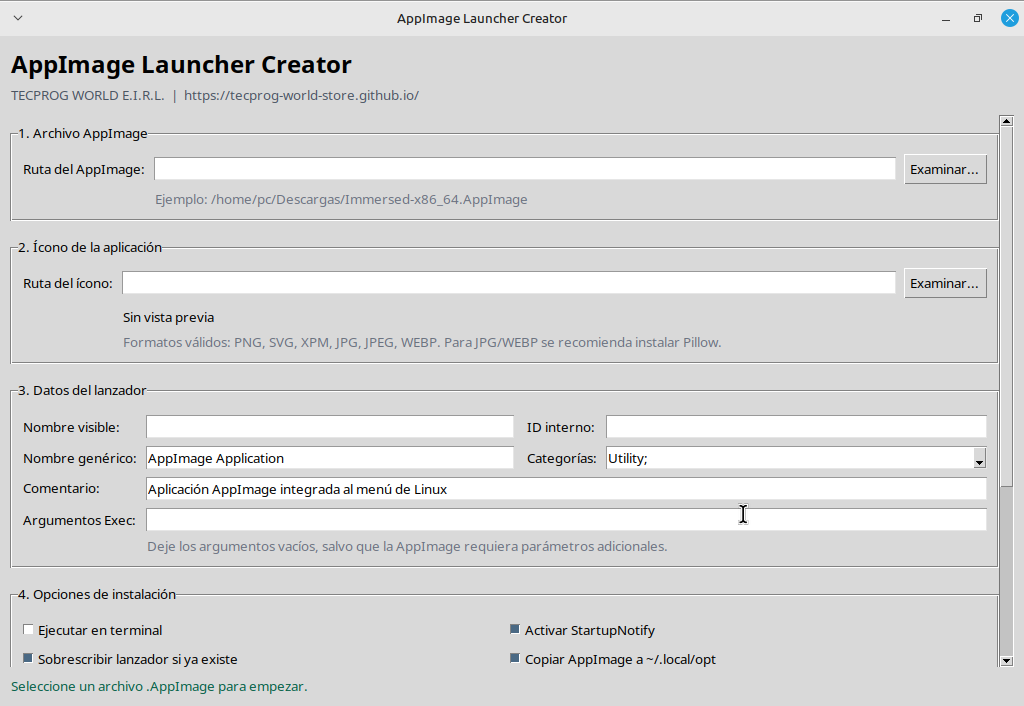
\includegraphics[width=0.98\textwidth]{figuras/appimage_launcher_creator_01.png}
    \caption{Interfaz principal de AppImage Launcher Creator para seleccionar el archivo AppImage, el ícono y los datos del lanzador.}
    \label{fig:gui-principal}
\end{figure}

La figura \ref{fig:gui-rutas} muestra la parte inferior del programa, donde se previsualizan las rutas de instalación y se encuentran los botones de validación, creación y prueba del lanzador.

\begin{figure}[H]
    \centering
    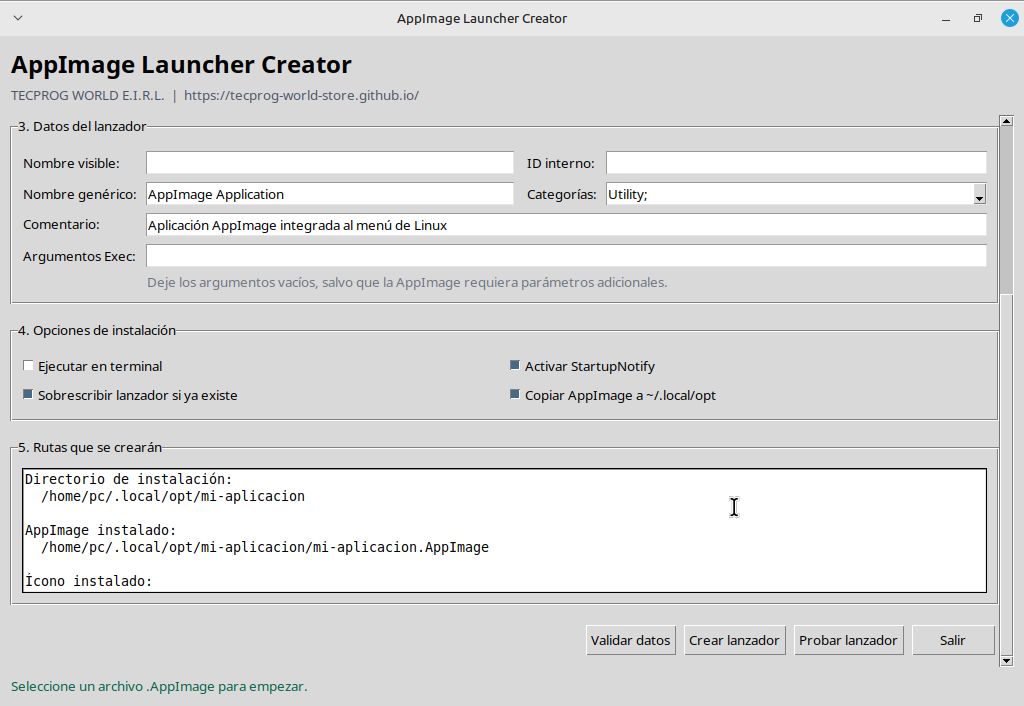
\includegraphics[width=0.98\textwidth]{figuras/appimage_launcher_creator_02.png}
    \caption{Sección de rutas generadas, opciones finales y botones principales del software.}
    \label{fig:gui-rutas}
\end{figure}

\section{Sección 1: Archivo AppImage}

La primera sección permite seleccionar el ejecutable portable de la aplicación. El botón \textbf{Examinar} abre el explorador de archivos del sistema para ubicar un archivo con extensión \texttt{.AppImage}. Al seleccionar el archivo, el software puede proponer automáticamente un nombre visible basado en el nombre del ejecutable.

\begin{lstlisting}[style=textstyle]
Ejemplo de ruta:
/home/pc/Descargas/Immersed-x86_64.AppImage
\end{lstlisting}

El archivo seleccionado debe existir y tener una extensión válida. Si el archivo no es reconocido como \texttt{AppImage}, la validación mostrará un mensaje de error.

\section{Sección 2: Ícono de la aplicación}

La segunda sección permite seleccionar la imagen que será usada como ícono en el menú de aplicaciones. El programa acepta formatos frecuentes como \texttt{PNG}, \texttt{SVG}, \texttt{XPM}, \texttt{JPG}, \texttt{JPEG} y \texttt{WEBP}. Para una integración más limpia en Linux Mint, se recomienda usar una imagen \texttt{PNG} cuadrada, por ejemplo de 256x256 o 512x512 píxeles.

\begin{lstlisting}[style=textstyle]
Ejemplo de ruta:
/home/pc/Descargas/immersed.png
\end{lstlisting}

Cuando el ícono es \texttt{PNG}, Tkinter suele mostrar una vista previa básica. Para otros formatos, puede ser necesario instalar Pillow.

\section{Sección 3: Datos del lanzador}

Esta sección define los metadatos del archivo \texttt{.desktop}. Estos campos son importantes porque determinan cómo se verá y clasificará la aplicación en el menú.

\subsection{Nombre visible}

El campo \textbf{Nombre visible} corresponde al nombre que aparecerá en el menú de Linux Mint. Por ejemplo:

\begin{lstlisting}[style=textstyle]
Immersed
QGIS Portable
Mi Aplicacion Cientifica
\end{lstlisting}

\subsection{ID interno}

El \textbf{ID interno} se usa para crear los nombres técnicos de carpetas y archivos. Debe ser corto, sin espacios y preferentemente en minúsculas.

\begin{lstlisting}[style=textstyle]
immersed
qgis-portable
mi-aplicacion-cientifica
\end{lstlisting}

Este identificador será usado para construir rutas como:

\begin{lstlisting}[style=textstyle]
~/.local/opt/immersed/
~/.local/share/applications/immersed.desktop
\end{lstlisting}

\subsection{Nombre genérico}

El campo \textbf{Nombre genérico} describe la clase de aplicación. Puede ser algo general como:

\begin{lstlisting}[style=textstyle]
AppImage Application
Remote Desktop Client
Scientific Software
Development Tool
\end{lstlisting}

\subsection{Categorías}

Las categorías permiten que el entorno gráfico ubique la aplicación en una sección del menú. Algunos ejemplos válidos son:

\begin{lstlisting}[style=textstyle]
Utility;
Network;RemoteAccess;Utility;
Development;
Graphics;
AudioVideo;
Office;
Education;
Science;Education;
System;
\end{lstlisting}

Para una aplicación como Immersed, una categoría razonable es:

\begin{lstlisting}[style=textstyle]
Network;RemoteAccess;Utility;
\end{lstlisting}

\subsection{Comentario}

El comentario describe brevemente la función de la aplicación. Este texto puede aparecer como ayuda contextual en algunos entornos de escritorio.

\begin{lstlisting}[style=textstyle]
Cliente Immersed para escritorio remoto, productividad y realidad virtual
\end{lstlisting}

\subsection{Argumentos Exec}

El campo \textbf{Argumentos Exec} debe dejarse vacío en la mayoría de casos. Solo se completa cuando la aplicación requiere parámetros adicionales al ejecutarse.

\begin{lstlisting}[style=textstyle]
Ejemplo común:
campo vacío

Ejemplo avanzado:
--no-sandbox
\end{lstlisting}

\section{Sección 4: Opciones de instalación}

La sección de opciones controla el comportamiento final del lanzador.

\subsection{Ejecutar en terminal}

Esta opción debe activarse solamente si la aplicación requiere abrirse dentro de una terminal. Para aplicaciones gráficas AppImage, normalmente se mantiene desactivada.

\subsection{Activar StartupNotify}

Esta opción permite que el escritorio muestre retroalimentación visual al iniciar la aplicación. Se recomienda mantenerla activada.

\subsection{Sobrescribir lanzador si ya existe}

Esta opción permite reemplazar un lanzador anterior con el mismo ID interno. Es útil cuando se desea actualizar una aplicación o corregir su ícono.

\subsection{Copiar AppImage a \texttt{\~{}/.local/opt}}

Esta opción copia el ejecutable AppImage a una ruta estable dentro del usuario. Se recomienda mantenerla activada porque evita depender de la carpeta \texttt{Descargas}.

\section{Sección 5: Rutas que se crearán}

El programa muestra una vista previa de las rutas que se generarán. Esto permite verificar el resultado antes de crear el lanzador.

\begin{lstlisting}[style=textstyle]
Directorio de instalacion:
  /home/pc/.local/opt/immersed

AppImage instalado:
  /home/pc/.local/opt/immersed/immersed.AppImage

Icono instalado:
  /home/pc/.local/share/icons/immersed.png

Lanzador .desktop:
  /home/pc/.local/share/applications/immersed.desktop
\end{lstlisting}

Estas rutas siguen una organización local del usuario y no requieren permisos de administrador.

\section{Botones principales}

\subsection{Validar datos}

El botón \textbf{Validar datos} revisa que el archivo \texttt{AppImage} exista, que el nombre visible no esté vacío, que el ID interno sea válido y que la imagen seleccionada tenga un formato permitido.

\subsection{Crear lanzador}

El botón \textbf{Crear lanzador} copia el AppImage, copia el ícono, genera el archivo \texttt{.desktop}, concede permisos y actualiza la base local de aplicaciones.

\subsection{Probar lanzador}

El botón \textbf{Probar lanzador} intenta ejecutar el acceso creado mediante:

\begin{lstlisting}[style=bashstyle]
gtk-launch nombre-del-id
\end{lstlisting}

Para el caso de Immersed:

\begin{lstlisting}[style=bashstyle]
gtk-launch immersed
\end{lstlisting}

\subsection{Salir}

El botón \textbf{Salir} cierra el programa.

\section{Ejemplo completo: crear lanzador para Immersed}

Para instalar Immersed como aplicación de menú, completar los campos así:

\begin{longtable}{>{\bfseries}p{5cm}p{10cm}}
\toprule
Campo & Valor recomendado \\
\midrule
Archivo AppImage & \texttt{/home/pc/Descargas/Immersed-x86\_64.AppImage} \\
Ícono & \texttt{/home/pc/Descargas/immersed.png} \\
Nombre visible & \texttt{Immersed} \\
ID interno & \texttt{immersed} \\
Nombre genérico & \texttt{Immersed Remote Desktop} \\
Categorías & \texttt{Network;RemoteAccess;Utility;} \\
Comentario & \texttt{Cliente Immersed para escritorio remoto, productividad y realidad virtual} \\
Argumentos Exec & vacío \\
\bottomrule
\end{longtable}

Luego presionar \textbf{Validar datos}, después \textbf{Crear lanzador} y finalmente buscar \textbf{Immersed} en el menú de aplicaciones.

\section{Estructura generada por el software}

Después de crear el lanzador, el sistema tendrá una estructura similar a la siguiente:

\begin{lstlisting}[style=textstyle]
/home/pc/.local/opt/immersed/
|-- immersed.AppImage

/home/pc/.local/share/icons/
|-- immersed.png

/home/pc/.local/share/applications/
|-- immersed.desktop
\end{lstlisting}

\section{Contenido típico de un archivo \texttt{.desktop}}

El lanzador generado tiene una estructura similar a:

\begin{lstlisting}[style=textstyle]
[Desktop Entry]
Version=1.0
Type=Application
Name=Immersed
GenericName=Immersed Remote Desktop
Comment=Cliente Immersed para escritorio remoto, productividad y realidad virtual
Exec="/home/pc/.local/opt/immersed/immersed.AppImage"
Icon=/home/pc/.local/share/icons/immersed.png
Terminal=false
StartupNotify=true
Categories=Network;RemoteAccess;Utility;
MimeType=
\end{lstlisting}

Este archivo permite que Linux Mint reconozca la aplicación y la muestre en el menú.

\section{Solución de problemas frecuentes}

\subsection{La aplicación no aparece en el menú}

Actualizar la base de datos de aplicaciones:

\begin{lstlisting}[style=bashstyle]
update-desktop-database ~/.local/share/applications
\end{lstlisting}

En XFCE, también puede reiniciarse el panel:

\begin{lstlisting}[style=bashstyle]
xfce4-panel -r
\end{lstlisting}

Si el problema continúa, cerrar sesión y volver a ingresar.

\subsection{El AppImage no abre}

Verificar que tenga permisos de ejecución:

\begin{lstlisting}[style=bashstyle]
chmod +x ~/.local/opt/immersed/immersed.AppImage
\end{lstlisting}

Ejecutarlo manualmente:

\begin{lstlisting}[style=bashstyle]
~/.local/opt/immersed/immersed.AppImage
\end{lstlisting}

\subsection{Error relacionado con FUSE}

Algunos AppImage requieren compatibilidad con FUSE. En Linux Mint moderno puede ser necesario instalar:

\begin{lstlisting}[style=bashstyle]
sudo apt update
sudo apt install libfuse2t64
\end{lstlisting}

\subsection{El ícono no aparece}

Verificar que el ícono exista:

\begin{lstlisting}[style=bashstyle]
ls -lh ~/.local/share/icons/immersed.png
\end{lstlisting}

Si se modificó el ícono, actualizar el lanzador o volver a crearlo con la opción de sobrescritura activada.

\subsection{El botón Probar lanzador falla}

Verificar que \texttt{gtk-launch} pueda ubicar el archivo:

\begin{lstlisting}[style=bashstyle]
gtk-launch immersed
\end{lstlisting}

Si no lo encuentra, revisar que exista:

\begin{lstlisting}[style=bashstyle]
ls -lh ~/.local/share/applications/immersed.desktop
\end{lstlisting}

\section{Buenas prácticas}

\begin{itemize}[leftmargin=1.2cm]
    \item Usar nombres de ID interno simples, sin espacios ni tildes.
    \item Mantener el AppImage instalado en \texttt{\~{}/.local/opt}.
    \item Usar íconos en formato \texttt{PNG} cuadrado para mayor compatibilidad.
    \item No eliminar manualmente archivos dentro de \texttt{\~{}/.local/opt} si el lanzador depende de ellos.
    \item Crear un respaldo del AppImage antes de actualizar una aplicación.
\end{itemize}

\section{Proyección técnica}

El software puede evolucionar hacia un paquete instalable \texttt{.deb}. Para ello, se recomienda definir un ícono oficial de la aplicación, instalar el ejecutable en \texttt{/usr/bin} o \texttt{/opt}, instalar su lanzador en \texttt{/usr/share/applications} y distribuir los recursos gráficos en \texttt{/usr/share/icons}. Esta evolución permitiría que \textit{AppImage Launcher Creator} se instale como una herramienta regular dentro de Linux Mint.

\section{Conclusión}

\textit{AppImage Launcher Creator} simplifica la integración de aplicaciones portables en Linux Mint al automatizar la creación de archivos \texttt{.desktop}, la copia de ejecutables y la asociación de íconos. La herramienta permite que usuarios técnicos y no técnicos organicen sus aplicaciones AppImage sin depender de la carpeta \texttt{Descargas} ni escribir manualmente configuraciones del menú. Este flujo mejora la trazabilidad del software instalado, reduce errores de ruta y facilita el uso cotidiano de aplicaciones portables dentro del escritorio Linux.

\section*{Contacto institucional}

\begin{longtable}{>{\bfseries}p{5cm}p{10cm}}
Empresa & TECPROG WORLD E.I.R.L. \\
RUC & 20608743252 \\
Actividad principal & Actividades de arquitectura e ingeniería y actividades conexas de consultoría técnica \\
Ubicación & San Martín de Porres, Lima, Perú \\
Sitio web & \url{https://tecprog-world-store.github.io/} \\
\end{longtable}

\end{document}
